\chapter{Results and Discussion}\label{chapter:results}

% Due to the huge amount of data, we will present the result of one design, specifically SV167-b5, and then compare it to the other desisng in the discussion. All the results can be find in
% TODO: REF APPENDIX
\section{Measurement results}
\subsection{Results of SV167-b5}
In \cref{fig:gainSV167} the result of the \qty{0}{\celsius} measurement can be seen. 

\begin{figure}
    \centering
    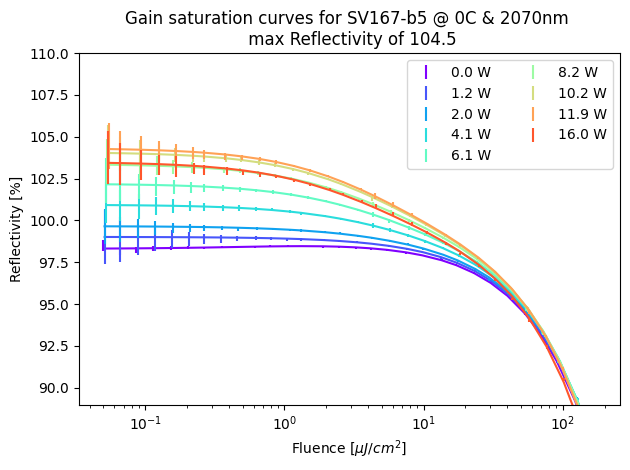
\includegraphics[width=10cm]{images/sv167-b5_0C.png}
    \caption{}
    \label{fig:gainSV167}
\end{figure}

